\clearpage
\section{Finding useful representations}
\label{sec:representations}
% EDITORIAL ADDITION: navigation or conceptual bridge
Choosing a variable was already part of constructing a model in section~\ref{sec:rates}.
The question now is how to represent a function, dataset, or biological shape so that its important structure becomes visible.
Fourier modes offered one example; normal modes and principal components offer others.
% Source: day5.tex:50; unit d5.1.0


% ============================================================

The way in which a problem is represented can determine which aspects of the problem become easy or difficult to see.
A useful representation exposes the structure that matters while suppressing details that are irrelevant to the question being asked.

% The same idea applies to how we describe ourselves.
% Labels such as ``physicist'' or ``biologist'' are only one possible representation and may hide much of the information that actually characterizes a person.


% ------------------------------------------------------------

% Source: day5.tex:61; unit d5.1.1
\subsection{Vectors as representations of biological objects}
\label{sec:vectors}

% ------------------------------------------------------------

Many complicated objects can be represented as vectors.
Once an object has been written as a vector, the tools of linear algebra can be used to compare objects, transform representations, and identify important directions of variation.

Examples include:

\begin{itemize}
    \item an image, represented by a vector of pixel intensities;
    \item a transcriptome, represented by a vector of gene-expression levels;
    \item a biological shape, represented by coordinates or by coefficients in a suitable basis, such as spherical harmonics or finite elements;
    \item a probability distribution, represented by the probabilities associated with each possible state.
\end{itemize}


% ------------------------------------------------------------

% EDITORIAL ADDITION: navigation or conceptual bridge
The Buri probability vector is developed alongside its experiment in section~\ref{sec:buri-vector}.
% Source: day3.tex:909; unit d3.7.0
\subsection{Approximating functions with simpler building blocks}
\label{sec:approximations}


% ============================================================

A complicated function or collection of data can often be represented approximately using simpler mathematical objects.
Different representations are useful in different situations.


% ------------------------------------------------------------

% EDITORIAL ADDITION: navigation or conceptual bridge
Taylor expansions use local derivatives; interpolation uses values at known points.
Their full explanations, worked examples, and interpolation figure are given in appendices~\ref{math:taylor} and~\ref{math:interpolation}.
% Source: day3.tex:1035; unit d3.7.3
\subsubsection{ReLU and piecewise-linear representations}
\label{sec:relu}

% ------------------------------------------------------------

A rectified linear unit, or ReLU, is a piecewise-linear function defined by

\[
    \boxed{\operatorname{ReLU}(x)=\max(0,x).}
\]

Equivalently,

\[
    \operatorname{ReLU}(x) =
    \begin{cases}
        0, & x<0, \\
        x, & x\geq0.
    \end{cases}\]

The function is therefore flat for negative inputs and linear for positive inputs.

ReLU functions are widely used as activation functions in neural networks.
Although a single ReLU is extremely simple, combinations of many ReLU units can produce complicated piecewise-linear functions.
Thus ReLUs provide another way of building a complicated function from simple components.


% ------------------------------------------------------------

% Source: day3.tex:1062; unit d3.7.4
\subsection{Least squares: choosing a representation from data}
\label{sec:least-squares}

% ------------------------------------------------------------

Least squares is a method for finding a model that best represents a collection of data.

Suppose we have measurements

\[
    (x_1,y_1), (x_2,y_2), \ldots, (x_N,y_N)
\]

and a model that predicts values

\[
    \hat{y}_i=f(x_i).
\]

The residual for measurement $i$ is the difference between the observed and predicted values,

\[
    r_i = y_i-\hat{y}_i.
\]

Least squares chooses the parameters of the model so that the sum of the squared residuals is as small as possible,

\[
    \boxed{\text{minimize} \qquad \sum_{i=1}^{N}\left(y_i-\hat{y}_i\right)^2.}
\]

Squaring the residuals prevents positive and negative errors from simply cancelling one another.
The result is the model that gives the smallest total squared discrepancy from the data according to this criterion.
% 
% 
\paragraph{Legendre, Gauss, and least squares}
Adrien-Marie Legendre published the method of least squares in 1805 as a practical method for extracting parameters from astronomical observations when there were more measurements than unknown quantities.
Carl Friedrich Gauss published his treatment in 1809 and claimed that he had used the method earlier, producing a lasting historical priority dispute between Gauss and Legendre \cite{stigler1981gauss}.
The method subsequently became fundamental for fitting mathematical models to noisy observations.

% \paragraph{Common idea}
\bigskip

These methods provide different ways of replacing something complicated by something simpler.
A Taylor expansion represents a function locally using a polynomial.
Linear interpolation represents the function between two known points using a straight line.
ReLU functions provide simple piecewise-linear building blocks from which more complicated functions can be constructed.
Least squares chooses the representation that best matches a collection of measurements according to a specified error measure.


% ============================================================

% Source: day5.tex:135; unit d5.2.0
\subsubsection{A straight-line fitting problem}
\label{sec:fit}


% ============================================================

Suppose we have $N$ data points
\[
    (x_1,y_1),(x_2,y_2),\ldots,(x_N,y_N)
\]
and wish to represent them by a straight line,
\[
    y=ax+b.
\]
For each data point, the residual between the observed and predicted value is
\[
    r_i=y_i-(ax_i+b).
\]
The least-squares method chooses $a$ and $b$ to minimize the sum of the squared residuals,
\[
    E(a,b)=\sum_{i=1}^{N}\left[y_i-(ax_i+b)\right]^2.
\]
This provides a quantitative definition of the ``best-fitting'' line.


% ------------------------------------------------------------

% Source: day5.tex:166; unit d5.2.1
\subsubsection{Why squares? Gaussian measurement noise}
\label{sec:gaussian-noise}

% ------------------------------------------------------------

One reason squared errors arise naturally is that measurement errors are often modeled as independent Gaussian random variables.

Suppose
\[
    y_i=ax_i+b+\epsilon_i,
\]
where
\[
    \epsilon_i\sim\mathcal{N}(0,\sigma^2).
\]
The probability density of observing $y_i$ for given $a$ and $b$ is then
\[
    p(y_i\mid x_i,a,b)=\frac{1}{\sqrt{2\pi\sigma^2}}\exp\left[-\frac{\left(y_i-ax_i-b\right)^2}{2\sigma^2}\right].
\]
Assuming that the errors of different measurements are independent, the likelihood of the complete dataset is
\[
    \mathcal{L}(a,b)=\prod_{i=1}^{N}p(y_i\mid x_i,a,b).
\]
Taking the logarithm converts the product into a sum,
\[
    \ln\mathcal{L}(a,b)=\text{constant}-\frac{1}{2\sigma^2}\sum_{i=1}^{N}\left[y_i-(ax_i+b)\right]^2.
\]
Maximizing the likelihood is therefore equivalent to minimizing
\[
    \sum_{i=1}^{N}\left[y_i-(ax_i+b)\right]^2.
\]

Thus least squares follows naturally from a model in which the measurement noise is independent and Gaussian with constant variance.


% ------------------------------------------------------------

% EDITORIAL ADDITION: navigation or conceptual bridge
The parameter calculation, normal equations, matrix representation, and explicit slope and intercept are retained in appendix~\ref{deriv:fit}.
% Source: day5.tex:307; unit d5.3.0
\subsection{Finding the right coordinates}
\label{sec:coordinates}


% ============================================================

A representation can be formally correct and still be inconvenient.
An important strategy in physics is therefore to search for coordinates in which the important structure of the problem becomes simple.


% ------------------------------------------------------------

% Source: day5.tex:315; unit d5.3.1
\subsubsection{Coupled oscillators and normal modes}
\label{sec:normal-modes}

% ------------------------------------------------------------

Consider two masses coupled by springs.

\begin{figure}[h!]
\centering
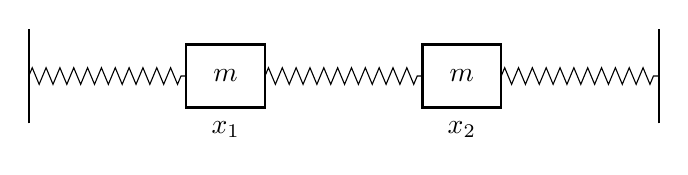
\begin{tikzpicture}

    \draw[thick] (0,0) -- (0,1.2);
    \draw[thick] (8,0) -- (8,1.2);

    \draw[decorate,decoration={zigzag,segment length=5pt,amplitude=3pt}] (0,0.6) -- (2,0.6);

    \draw[thick] (2,0.2) rectangle (3,1.0);
    \node at (2.5,0.6) {$m$};

    \draw[decorate,decoration={zigzag,segment length=5pt,amplitude=3pt}] (3,0.6) -- (5,0.6);

    \draw[thick] (5,0.2) rectangle (6,1.0);
    \node at (5.5,0.6) {$m$};

    \draw[decorate,decoration={zigzag,segment length=5pt,amplitude=3pt}] (6,0.6) -- (8,0.6);

    \node[below] at (2.5,0.15) {$x_1$};
    \node[below] at (5.5,0.15) {$x_2$};

\end{tikzpicture}
\caption{Two coupled oscillators.
The individual displacements $x_1$ and $x_2$ provide one coordinate system, while the normal modes provide another.}
\end{figure}

The individual mass displacements $x_1$ and $x_2$ are natural coordinates, but their equations of motion are coupled.

For a symmetric system, more useful coordinates are the combinations
\[
    q_{+}=\frac{x_1+x_2}{\sqrt{2}}
\]
and
\[
    q_{-}=\frac{x_1-x_2}{\sqrt{2}}.
\]
The coordinate $q_{+}$ describes the mode in which the masses move together.
The coordinate $q_{-}$ describes the mode in which they move oppositely.
These are the normal modes of the system.
In normal-mode coordinates, the coupled problem can be decomposed into independent motions.
This illustrates the importance of finding coordinates adapted to the structure of the problem.


% ============================================================

% Source: day5.tex:371; unit d5.3.2
\subsubsection{Covariance: which variables fluctuate together?}
\label{sec:covariance}

% ============================================================

The variance of a variable $x$ measures its fluctuations around its mean,
\[
    \operatorname{Var}(x)=\left\langle\left(x-\langle x\rangle\right)^2\right\rangle.
\]
Expanding the square gives
\[
    \operatorname{Var}(x)=\langle x^2\rangle-\langle x\rangle^2.
\]
For two variables $x_1$ and $x_2$, the covariance is
\[
    \operatorname{Cov}(x_1,x_2)=\left\langle\left(x_1-\langle x_1\rangle\right)\left(x_2-\langle x_2\rangle\right)\right\rangle.
\]
The covariance matrix for two variables is
\[
    C=
    \begin{pmatrix}
        \left\langle\left(x_1-\langle x_1\rangle\right)^2\right\rangle &
        \left\langle\left(x_1-\langle x_1\rangle\right)\left(x_2-\langle x_2\rangle\right)\right\rangle \\
        \left\langle\left(x_1-\langle x_1\rangle\right)\left(x_2-\langle x_2\rangle\right)\right\rangle &
        \left\langle\left(x_2-\langle x_2\rangle\right)^2\right\rangle
    \end{pmatrix}.
\]
The diagonal entries describe the variance of each coordinate.
The off-diagonal entries describe how fluctuations in different coordinates are correlated.


% ============================================================

% Source: day5.tex:409; unit d5.3.3
\subsubsection{Principal component analysis}
\label{sec:pca}

% ============================================================

Principal component analysis, or PCA, provides a systematic way to find coordinates that capture the dominant variation in a dataset \cite{pearson1901liii,hotelling1933analysis}.

For variables collected into a vector $\mathbf{x}$, define the covariance matrix
\[
    C_{ij}=\left\langle\left(x_i-\langle x_i\rangle\right)\left(x_j-\langle x_j\rangle\right)\right\rangle.
\]
The principal components are the eigenvectors of this matrix,
\[
    C\mathbf{v}_{\mu}=\lambda_{\mu}\mathbf{v}_{\mu}.
\]
The eigenvectors $\mathbf{v}_{\mu}$ define new coordinate directions.
The corresponding eigenvalues $\lambda_{\mu}$ measure the variance of the data along those directions.

The first principal component is the direction along which the data vary most.
The second is the orthogonal direction containing the next-largest variance, and so on.

If only a few eigenvalues are large, a high-dimensional dataset can be represented accurately using only a few principal components.
PCA therefore provides both a change of coordinates and a method for dimensionality reduction.


% ============================================================

% Source: day5.tex:436; unit d5.4
\subsection{The eigenworm: low-dimensional shape and behavior}
\label{sec:eigenworm}


% ============================================================

A biological example of finding useful coordinates is the quantitative analysis of \textit{Caenorhabditis elegans} posture and locomotion by Stephens et al.\ \cite{stephens2008dimensionality}.
Their goal was to determine whether the apparently complicated set of worm postures could be represented using only a few collective coordinates.

A simplified image-analysis and PCA pipeline is:
\begin{enumerate}[start=0]
    \item Parse the image data.
    \item Segment the worm from the image background.
    \item Skeletonize the worm to determine its centerline.
    \item Fit or sample a smooth contour along the centerline.
    \item Compute the tangent angle along the body for every recorded time.
    \item Arrange the tangent-angle data as a function of body position and time.
    \item Compute the covariance matrix of the angular fluctuations.
    \item Perform principal component analysis.
    \item Decompose each observed posture into the resulting eigenmodes.
\end{enumerate}

Let $\theta(s,t)$ denote the tangent angle at position $s$ along the worm body at time $t$.
After removing the overall orientation of the worm, a posture can be represented by the set of angles along its body (Fig~\ref{fig:worm_shape}).

\begin{figure}[h]
    \centering
    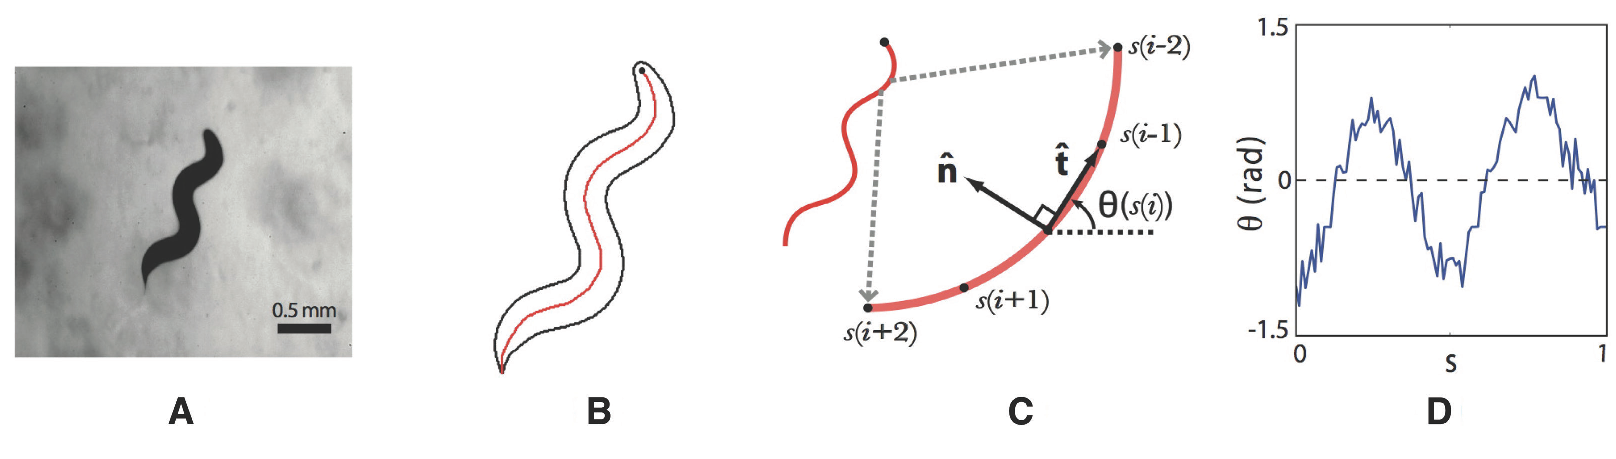
\includegraphics[width=\linewidth]{figures/eigenworms_fig1_edited.pdf}
    \caption{Representing the shape of \textit{C. elegans}.
    A raw microscopy image of the worm is reduced to a curve along its centerline.
    Position along the body is described by the normalized arclength $s$, while the local tangent angle $\theta(s)$ records the orientation of each body segment.
    Subtracting the mean angle removes the overall orientation of the animal, producing an intrinsic description of posture that can be compared across images.
    Adapted from Figure~1 of Stephens et al.\ \cite{stephens2008dimensionality}; panels have been rearranged.}
    \label{fig:worm_shape}
\end{figure}

The covariance between two body positions $s$ and $s'$ is
\[
    C(s,s')=\left\langle\left[\theta(s,t)-\langle\theta(s,t)\rangle_t\right]\left[\theta(s',t)-\langle\theta(s',t)\rangle_t\right]\right\rangle_t,
\]
where $\langle\cdot\rangle_t$ denotes an average over the recorded postures.
The eigenvectors of this covariance matrix satisfy
\[
    \sum_{s'}C(s,s')u_{\mu}(s')=\lambda_{\mu}u_{\mu}(s).
\]
These principal components are called \emph{eigenworms}.
The worm shape can then be represented approximately as
\[
    \theta(s,t)\approx\sum_{\mu=1}^{K}a_{\mu}(t)u_{\mu}(s).
\]


Stephens et al.\ found that four eigenworms account for approximately $95\%$ of the observed variance in worm shapes (Fig.~\ref{fig:eigenworms}) \cite{stephens2008dimensionality}.

\begin{figure}[h]
    \centering
    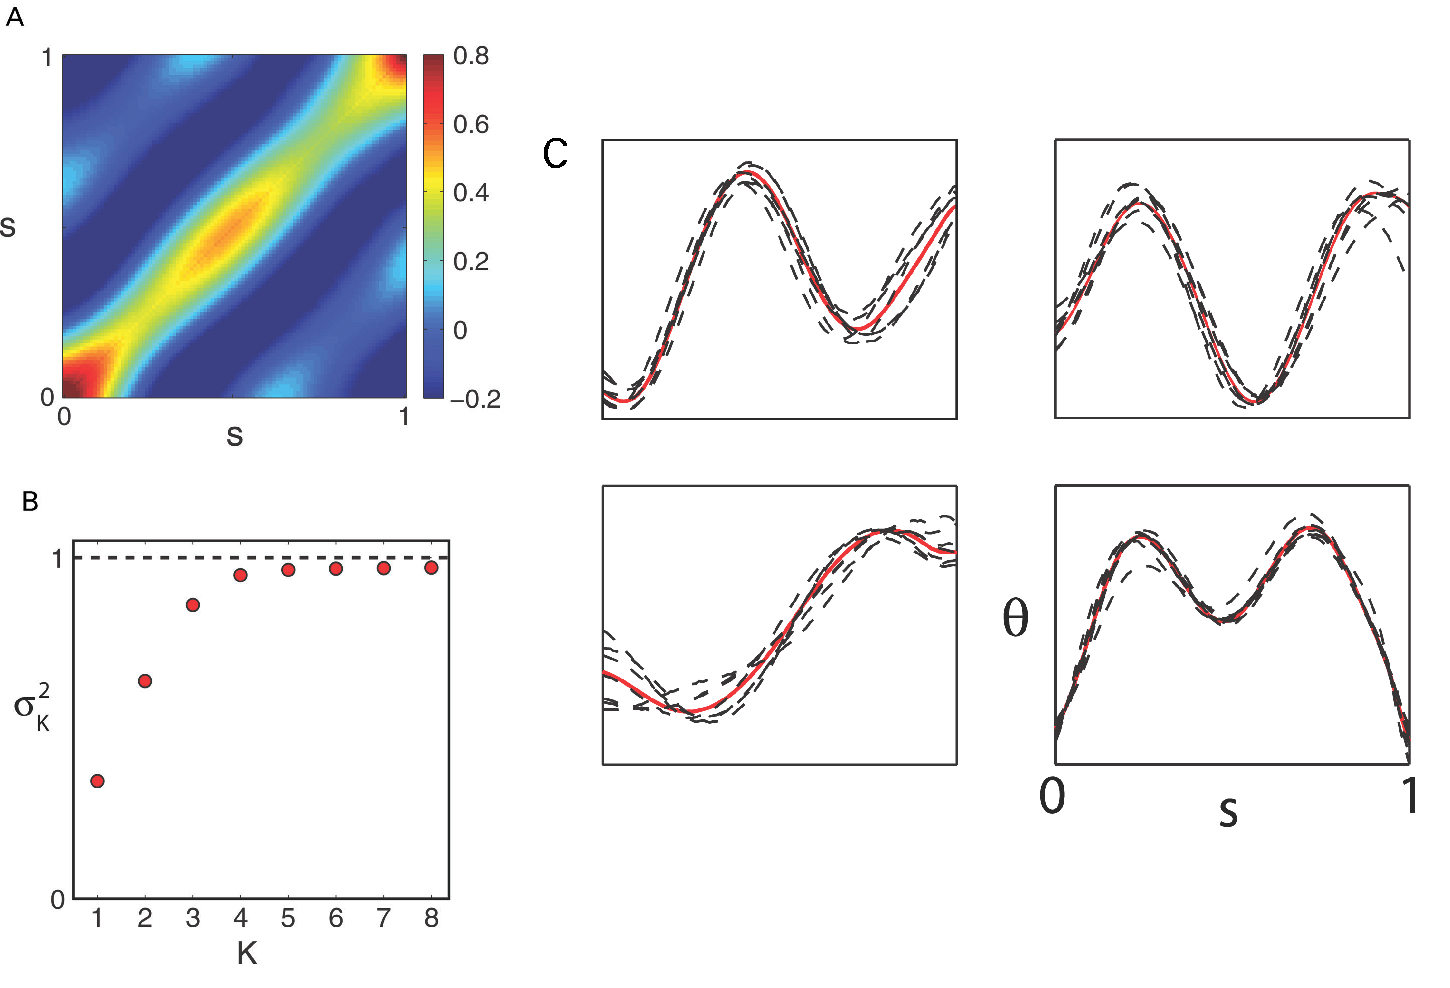
\includegraphics[width=0.8\linewidth]{figures/eigenworms_fig2_edited.pdf}
    \caption{Covariance, dimensionality, and the eigenworms.
    (A) The covariance matrix $C(s,s')$ measures how tangent-angle fluctuations at different positions along the worm body vary together.
    Its smooth structure indicates that the observed posture fluctuations may be described by a small number of collective modes.
    (B) The cumulative fraction of posture variance captured by the first $K$ modes rises rapidly; four modes account for approximately $95\%$ of the total variance.
    (C) The corresponding eigenvectors of the covariance matrix are the eigenworms $u_{\mu}(s)$.
    Population-averaged eigenworms are shown in red, while eigenworms calculated for individual animals are shown in black, demonstrating that the dominant modes are reproducible across worms.
    Adapted from Figure~2A--C of Stephens et al.\ \cite{stephens2008dimensionality}.}
    \label{fig:eigenworms}
\end{figure}

Thus an object initially represented using roughly one hundred local angular coordinates can be represented, to good approximation, by only four mode amplitudes,
\[
    \mathbf{a}(t)=
    \begin{pmatrix}
        a_1(t) \\
        a_2(t) \\
        a_3(t) \\
        a_4(t)
    \end{pmatrix}.
\]

The important result is not merely data compression.
The new coordinates provide a compact description of the behavior and dynamics of the animal.


\subsubsection{Geometric phase and locomotion}

Rieser et al.\ used a geometric-phase framework to connect cyclic changes in body shape to locomotion in undulating animals operating in highly damped environments \cite{rieser2024geometric}.
Periodic locomotion can be represented as a closed trajectory through a low-dimensional space of body shapes.
The coordinates of this space describe how much of each shape mode is present at a given time.

As an animal cycles through a sequence of shapes, it traces a loop through shape space.
In the friction-dominated regimes considered in the study, the geometry of this loop predicts the net displacement accumulated during a locomotor cycle.
Thus an appropriate low-dimensional representation can expose a direct relationship between body-shape dynamics and locomotor performance.

% ============================================================

% EDITORIAL ADDITION: navigation or conceptual bridge
% The eigenworm reconstruction above uses the centered, orientation-adjusted shape convention.
% If a nonzero mean shape is retained, add it explicitly to the mode expansion.
% Normal modes diagonalize a dynamical operator, whereas PCA diagonalizes a covariance matrix; these two operators answer different questions.
